% *******************************************************
% *******************************************************
%
% Copyright 2014 Benjamin Tovar Cisneros <https://github.com/TATABOX42>
%
% This program is free software; you can redistribute it and/or modify
% it under the terms of the GNU General Public License as published by
% the Free Software Foundation; either version 2 of the License, or
% (at your option) any later version.
%
% This program is distributed in the hope that it will be useful,
% but WITHOUT ANY WARRANTY; without even the implied warranty of
% MERCHANTABILITY or FITNESS FOR A PARTICULAR PURPOSE.  See the
% GNU General Public License for more details.
%
% You should have received a copy of the GNU General Public License
% along with this program; if not, write to the Free Software
% Foundation, Inc., 51 Franklin Street, Fifth Floor, Boston,
% MA 02110-1301, USA.
%
% *******************************************************
% contact: benjamin.tovarcis@gmail.com
% *******************************************************

% set document class
\documentclass[a4paper,12pt]{report}
% load document packages
\usepackage{class//thesis}
% load space package
\usepackage{setspace}

% *******************************
% set variables
% *******************************

	% set the author's name (First Middle ­Last ­Name)
	\newcommand{\authorName}{Arthur Philip Dent}
	% set the author's school program
	\newcommand{\schoolProgram}{Master of Science in Intelligent Systems}
	% set the thesis name
	\newcommand{\thesisTitle}{
								APPLICATION OF EVOLUTIONARY ALGORITHMS 
								TO SOLVE THE INFINITE MONKEY THEOREM
	  					}

	% set the school name
	\newcommand{\schoolName}{Instituto Tecnológico y de Estudios Superiores de Monterrey}
	\newcommand{\schoolCampus}{Campus Monterrey}
	% set the department name
	\newcommand{\schoolDepartment}{School of Engineering and Sciences}
	% set school other details:
	\newcommand{\schoolPlace}{Monterrey, N.L.}
	\newcommand{\thesisDate}{December, 2014}
	\newcommand{\thesisYear}{2014}
	% extra stuff
	\author{\authorName}
	\title{\thesisTitle}

	% *******************************
	% set variables for thesis committee 
	% *******************************

	% 1st adviser variables (Dr. First Middle ­Last ­Name)
	\newcommand{\firstAdvisorName}{Dr. Principal Adviser}
	\newcommand{\firstAdvisorSchoolName}{\schoolName}
	\newcommand{\firstAdvisorSchoolDepartment}{\schoolDepartment}
	\newcommand{\firstAdvisorSchoolPlace}{\schoolPlace}

	% 2nd adviser variables (Dr. First Middle ­Last ­Name)
	\newcommand{\secondAdvisorName}{Dr. Adviser Number Two}
	\newcommand{\secondAdvisorSchoolName}{\schoolName}
	\newcommand{\secondAdvisorSchoolPlace}{\schoolPlace}

	% 3rd adviser variables (Dr. First Middle ­Last ­Name)
	\newcommand{\thirdAdvisorName}{Dr. Adviser Number Three}
	\newcommand{\thirdAdvisorSchoolName}{University of California, San Diego}
	\newcommand{\thirdAdvisorSchoolPlace}{San Diego, United States of America}

	% Program director variables (Dr. First Middle ­Last ­Name)
	\newcommand{\programDirectorName}{Dr. Jorge Welti Chanes}
	\newcommand{\programDirectorRole}{Associate Dean of Graduate Studies}

% *******************************************************
% *******************************************************
% Begin the document 
% NOTE: Do not move unless you want to change
% the order of chapters.
% *******************************************************
% *******************************************************

\begin{document}
	% import thesis cover: 
		\thispagestyle{empty} 
		%
% Copyright 2014 Benjamin Tovar Cisneros <https://github.com/TATABOX42>
%
% This program is free software; you can redistribute it and/or modify
% it under the terms of the GNU General Public License as published by
% the Free Software Foundation; either version 2 of the License, or
% (at your option) any later version.
%
% This program is distributed in the hope that it will be useful,
% but WITHOUT ANY WARRANTY; without even the implied warranty of
% MERCHANTABILITY or FITNESS FOR A PARTICULAR PURPOSE.  See the
% GNU General Public License for more details.
%
% You should have received a copy of the GNU General Public License
% along with this program; if not, write to the Free Software
% Foundation, Inc., 51 Franklin Street, Fifth Floor, Boston,
% MA 02110-1301, USA.
%

\begin{center}\large
    \textbf{\schoolName}\\
    \textbf{\schoolCampus}\\
    \textbf{\schoolDepartment}\\
\end{center}

%%%%%%%%%%%%%
\begin{center}
\end{center}
%%%%%%%%%%%%%

\begin{figure}[h!tb]
    \begin{center}
        
\includegraphics[width=0.7\columnwidth]{format/logo_TEC.png}
    \end{center}
\end{figure}

\begin{center}
    \textbf{\thesisTitle}
\end{center}

%%%%%%%%%%%%%
\begin{center}
\end{center}
%%%%%%%%%%%%%

\begin{center}
    \textbf{A thesis presented by:}
\end{center}

\begin{center}
    \textbf{\authorName}
\end{center}


%%%%%%%%%%%%%
\begin{center}
\end{center}
%%%%%%%%%%%%%

\begin{center}
    \textbf{Submitted to the
    School of Engineering and Sciences \\
    in partial fulfillment of the requirements for the degree of}
\end{center}

\begin{center}
    \textbf{\schoolProgram}
\end{center}

\null
\vfill

\begin{center}
    \textbf{\schoolPlace} 
\end{center}

\begin{center}
    \textbf{\thesisDate} 
\end{center}

 
		\newpage
	% load thesis committee:
		\thispagestyle{empty} 
		%
% Copyright 2014 Benjamin Tovar Cisneros <https://github.com/TATABOX42>
%
% This program is free software; you can redistribute it and/or modify
% it under the terms of the GNU General Public License as published by
% the Free Software Foundation; either version 2 of the License, or
% (at your option) any later version.
%
% This program is distributed in the hope that it will be useful,
% but WITHOUT ANY WARRANTY; without even the implied warranty of
% MERCHANTABILITY or FITNESS FOR A PARTICULAR PURPOSE.  See the
% GNU General Public License for more details.
%
% You should have received a copy of the GNU General Public License
% along with this program; if not, write to the Free Software
% Foundation, Inc., 51 Franklin Street, Fifth Floor, Boston,
% MA 02110-1301, USA.
%

\begin{center}\large
    \textbf{\schoolName}\\
    \textbf{\schoolCampus}\\
    \textbf{\schoolDepartment}\\
\end{center}

The  committee  members,  hereby,  certify  that  have  read  the  
thesis  presented  by \authorName\ and that it is fully 
adequate in scope and quality as a partial 
requirement  for  the  degree  of  \schoolProgram.

%%%%%%%%%%%%%
\begin{center}
\end{center}
%%%%%%%%%%%%%

\begin{center}
        \textbf{THESIS COMMITTEE}
\end{center}


\begin{flushright}
        \vspace{1cm}
        \underline{\hspace{8cm}} \\ 
        % -------------------------
        \MakeUppercase{\firstAdvisorName} \\
        \firstAdvisorSchoolName \\
        \firstAdvisorSchoolDepartment \\
        \firstAdvisorSchoolPlace \\
        Principal Adviser \\
        % -------------------------
\end{flushright}

\begin{flushright}
        \vspace{1cm}
        \underline{\hspace{8cm}}  \\
        % -------------------------
        \MakeUppercase{\secondAdvisorName} \\
        \secondAdvisorSchoolName \\
        \secondAdvisorSchoolPlace \\
        Committee Member \\
        % -------------------------
\end{flushright}

\begin{flushright}
        \vspace{1cm} 
        \underline{\hspace{8cm}} \\
        % -------------------------
        \MakeUppercase{\thirdAdvisorName} \\
        \thirdAdvisorSchoolName \\
        \thirdAdvisorSchoolPlace \\
        Committee Member \\
        % -------------------------
\end{flushright}

\begin{center}
        \vspace{1cm}
        \underline{\hspace{8cm}} \\
        % -------------------------
        \MakeUppercase{\programDirectorName} \\
        \programDirectorRole \\
        \schoolDepartment
        % -------------------------     
\end{center}

\null
\vfill

\begin{center}
    \textbf{\schoolPlace}, \textbf{\thesisDate} 
\end{center}





 
		%
% Copyright 2014 Benjamin Tovar Cisneros <https://github.com/TATABOX42>
%
% This program is free software; you can redistribute it and/or modify
% it under the terms of the GNU General Public License as published by
% the Free Software Foundation; either version 2 of the License, or
% (at your option) any later version.
%
% This program is distributed in the hope that it will be useful,
% but WITHOUT ANY WARRANTY; without even the implied warranty of
% MERCHANTABILITY or FITNESS FOR A PARTICULAR PURPOSE.  See the
% GNU General Public License for more details.
%
% You should have received a copy of the GNU General Public License
% along with this program; if not, write to the Free Software
% Foundation, Inc., 51 Franklin Street, Fifth Floor, Boston,
% MA 02110-1301, USA.
%

\thispagestyle{empty} % delete page number
\begin{center}
	\textbf{Declaration of Authorship}
\end{center}

	I, \authorName\, declare that this thesis titled, \thesisTitle\ and the 
	work presented in it are my own. I confirm that:

%%%%%%%%%%%%%
\begin{center}
\end{center}
%%%%%%%%%%%%%

\begin{itemize}
	\item This work was done wholly or mainly while in candidature for a research degree 
	at this University.
	\item Where any part of this thesis has previously been submitted for a degree or any 
	other qualification at this University or any other institution, this has been clearly 
	stated.
	\item Where I have consulted the published work of others, this is always clearly 
	attributed.
	\item Where I have quoted from the work of others, the source is always given. With 
	the exception of such quotations, this thesis is entirely my own work.
	\item I have acknowledged all main sources of help.
	\item Where the thesis is based on work done by myself jointly with others, I have 
	made clear exactly what was done by others and what I have contributed myself.
\end{itemize}

%%%%%%%%%%%%%
\begin{center}
\end{center}
%%%%%%%%%%%%%

\begin{flushright}
        \vspace{1 cm}
        \underline{\hspace{8cm}} \\ 
        % -------------------------
        \MakeUppercase{\authorName} \\
        \schoolPlace, \thesisDate
        % -------------------------
\end{flushright}

\null
\vfill

\begin{center}
	{@}\thesisYear\ by \authorName \\
	All rights reserved
\end{center}
 
		\newpage
	% set the numeric indexing to be roman
		\pagestyle{headings}
		\setcounter{page}{1}
		\pagenumbering{roman}
	% load dedicatory page
		\section*{Dedicatory}
\textit{To my family and friends}


	% load acknowledgments page
	  \section*{Acknowledgments}

%%%%%%%%%%%%%
\begin{center}
\end{center}
%%%%%%%%%%%%%


To my principal adviser \firstAdvisorName\ for his friendship 
and support along this work. 
\\
\\
To my family and friends


%%%%%%%%%%%%%
\begin{center}
\end{center}
%%%%%%%%%%%%%

\begin{flushright}  
	\MakeUppercase{\authorName}
\end{flushright}  

\schoolName 
\\
\thesisDate


	% Insert blank page
    \clearpage
		% \thispagestyle{empty}
		\hfill
		\clearpage
	%%%%%%%%%%%%%%%%%%%%%%%%%%%%%%%%%%%%%%%%%%%%%%%%%%%%%%%%%%%%%%%%%%%%%%%%%%%%%%%%
	% include abstract
		% ***************************************
% ***************************************
\chapter*{Abstract} \label{abstract}
\addcontentsline{toc}{chapter}{Abstract}
% ***************************************
% ***************************************

\begin{center}\large
    \textbf{\thesisTitle}\\
\end{center}

%%%%%%%%%%%%%
\begin{center}
\end{center}
%%%%%%%%%%%%%

\begin{center}
    \authorName\\
    \schoolName, \thesisYear\\
\end{center}

\begin{center}
    Principal adviser: \firstAdvisorName\\
\end{center}


%%%%%%%%%%%%%
\begin{center}
\end{center}
%%%%%%%%%%%%%


The infinite monkey theorem states that a monkey hitting keys at random on a typewriter keyboard for an infinite amount of time will almost surely type a given text, such as the complete works of William Shakespeare.
\\
\\
In this context, \textit{almost surely} is a mathematical term with a precise meaning, and the \textit{monkey} is not an actual monkey, but a metaphor for an abstract device that produces an endless random sequence of letters and symbols. One of the earliest instances of the use of the \textit{monkey metaphor} is that of French mathematician Émile Borel in 1913 \cite{borel1913mecanique}, but the earliest instance may be even earlier. The relevance of the theorem is questionable—the probability of a universe full of monkeys typing a complete work such as Shakespeare's Hamlet is so tiny that the chance of it occurring during a period of time hundreds of thousands of orders of magnitude longer than the age of the universe is extremely low (but technically not zero).
\\
\\
Variants of the theorem include multiple and even infinitely many typists, and the target text varies between an entire library and a single sentence. The history of these statements can be traced back to Aristotle's On Generation and Corruption and Cicero's De natura deorum (On the Nature of the Gods), through Blaise Pascal and Jonathan Swift, and finally to modern statements with their iconic simians and typewriters. In the early 20th century, Émile Borel and Arthur Eddington used the theorem to illustrate the timescales implicit in the foundations of statistical mechanics \cite{wikiMonkeys}.


	% list of figures
		\listoffigures
		\addcontentsline{toc}{chapter}{List of Figures}
		\newpage
	% list of tables
		\listoftables
		\addcontentsline{toc}{chapter}{List of Tables}
		\newpage
	% Index of contents
		{\pagestyle{plain}
		\tableofcontents
		\cleardoublepage}
		\newpage
	%%%%%%%%%%%%%%%%%%%%%%%%%%%%%%%%%%%%%%%%%%%%%%%%%%%%%%%%%%%%%%%%%%%%%%%%%%%%%%%%
	% change the numeration of pages to Arabic starting from number 1
		\pagestyle{headings}
		\setcounter{page}{1}
		\pagenumbering{arabic}
		\newpage
	%%%%%%%%%%%%%%%%%%%%%%%%%%%%%%%%%%%%%%%%%%%%%%%%%%%%%%%%%%%%%%%%%%%%%%%%%%%%%%%%

	% set space to one and half spacing:  
	\onehalfspacing

	% import text:
	% ********************** PART 1
		% ***************************************
% ***************************************
\chapter{Introduction} \label{introduction}
% ***************************************
% ***************************************

The infinite monkey theorem states that a monkey hitting keys at random on a typewriter keyboard for an infinite amount of time will almost surely type a given text, such as the complete works of William Shakespeare.
\\
\\
In this context, \textit{almost surely} is a mathematical term with a precise meaning, and the \textit{monkey} is not an actual monkey, but a metaphor for an abstract device that produces an endless random sequence of letters and symbols. One of the earliest instances of the use of the \textit{monkey metaphor} is that of French mathematician Émile Borel in 1913 \cite{borel1913mecanique}, but the earliest instance may be even earlier. The relevance of the theorem is questionable—the probability of a universe full of monkeys typing a complete work such as Shakespeare's Hamlet is so tiny that the chance of it occurring during a period of time hundreds of thousands of orders of magnitude longer than the age of the universe is extremely low (but technically not zero).
\\
\\
Variants of the theorem include multiple and even infinitely many typists, and the target text varies between an entire library and a single sentence. The history of these statements can be traced back to Aristotle's On Generation and Corruption and Cicero's De natura deorum (On the Nature of the Gods), through Blaise Pascal and Jonathan Swift, and finally to modern statements with their iconic simians and typewriters. In the early 20th century, Émile Borel and Arthur Eddington used the theorem to illustrate the timescales implicit in the foundations of statistical mechanics \cite{wikiMonkeys}.


% *******************************************
\section{Justification} \label{justification}
% *******************************************

Solving this problems is likely to solve another monkey problems.

% *******************************************
\section{Hypothesis} \label{hypothesis}
% *******************************************

Electronic simulated monkeys are likely to learn to write Shakespeare.

% *******************************************
\section{Objectives} \label{objectives}
% *******************************************

The general objective is to propose, implement, and characterize a model to solve the infinite monkey problem.
\\
\\
Specific objectives are listed below:

\begin{enumerate}
    \item Propose a model to solve the infinite monkey problem.
    \item Make them read Shakespeare.
    \item Make then write like Shakespeare.
\end{enumerate}


% *********************************************************
\section{Thesis contributions} \label{thesis_contributions}
% *********************************************************

The present work contributes with a mathematical and computational model to study 
perturbations in time and space given the modeling of probabilistic monkeys.

\begin{itemize}
	\item Construct a monkey database.
	\item Select equation parameters to model monkey performance.
	\item Run spelling-bee contests with monkeys.
\end{itemize}


% ***************************
\section{Thesis organization}
% ***************************

The organization of this thesis is as follows: Chapter \ref{background} introduces to basic concepts in monkey theory. In chapter \ref{materials_and_methods}, the materials and methods are shown. This chapter comprises the source and describes each datasets employed. The results, discussion,  conclusions and future work are shown in chapters \ref{results}, \ref{discussion} and \ref{conclusions} respectively.

		% ***************************************
% ***************************************
\chapter{Background} \label{background}
% ***************************************
% ***************************************

Through this chapter, a short 
introduction to the infinite monkey theorem is presented

% ******************************************************************************    
\section{Monkeys as complex systems}
% ******************************************************************************    

The infinite monkey theorem states that a monkey hitting keys at random on a typewriter keyboard for an infinite amount of time will almost surely type a given text, such as the complete works of William Shakespeare.
\\
\\
In this context, \textit{almost surely} is a mathematical term with a precise meaning, and the \textit{monkey} is not an actual monkey, but a metaphor for an abstract device that produces an endless random sequence of letters and symbols. One of the earliest instances of the use of the \textit{monkey metaphor} is that of French mathematician Émile Borel in 1913 \cite{borel1913mecanique}, but the earliest instance may be even earlier. The relevance of the theorem is questionable—the probability of a universe full of monkeys typing a complete work such as Shakespeare's Hamlet is so tiny that the chance of it occurring during a period of time hundreds of thousands of orders of magnitude longer than the age of the universe is extremely low (but technically not zero).
\\
\\
Variants of the theorem include multiple and even infinitely many typists, and the target text varies between an entire library and a single sentence. The history of these statements can be traced back to Aristotle's On Generation and Corruption and Cicero's De natura deorum (On the Nature of the Gods), through Blaise Pascal and Jonathan Swift, and finally to modern statements with their iconic simians and typewriters. In the early 20th century, Émile Borel and Arthur Eddington used the theorem to illustrate the timescales implicit in the foundations of statistical mechanics \cite{wikiMonkeys}.

%%%%%%%%%%%%%%%%%%%%%%%%%%%%%%%%%%%%%%%%%%%%%%%%%%%%%%%%%%%%%%%%%%%%%%%%%%%%%%%%
\section{Summarizing notes} 
%%%%%%%%%%%%%%%%%%%%%%%%%%%%%%%%%%%%%%%%%%%%%%%%%%%%%%%%%%%%%%%%%%%%%%%%%%%%%%%%

In synthesis, we have briefly presented how monkeys  
works to form complex interaction networks. 



	% % ********************** PART 2
		% ***************************************
% ***************************************
\chapter{Materials and methods} \label{materials_and_methods}
% ***************************************
% ***************************************

The infinite monkey theorem states that a monkey hitting keys at random on a typewriter keyboard for an infinite amount of time will almost surely type a given text, such as the complete works of William Shakespeare.
\\
\\
In this context, \textit{almost surely} is a mathematical term with a precise meaning, and the \textit{monkey} is not an actual monkey, but a metaphor for an abstract device that produces an endless random sequence of letters and symbols. One of the earliest instances of the use of the \textit{monkey metaphor} is that of French mathematician Émile Borel in 1913 \cite{borel1913mecanique}, but the earliest instance may be even earlier. The relevance of the theorem is questionable—the probability of a universe full of monkeys typing a complete work such as Shakespeare's Hamlet is so tiny that the chance of it occurring during a period of time hundreds of thousands of orders of magnitude longer than the age of the universe is extremely low (but technically not zero).
\\
\\
Variants of the theorem include multiple and even infinitely many typists, and the target text varies between an entire library and a single sentence. The history of these statements can be traced back to Aristotle's On Generation and Corruption and Cicero's De natura deorum (On the Nature of the Gods), through Blaise Pascal and Jonathan Swift, and finally to modern statements with their iconic simians and typewriters. In the early 20th century, Émile Borel and Arthur Eddington used the theorem to illustrate the timescales implicit in the foundations of statistical mechanics \cite{wikiMonkeys}.

% insert figure
\begin{figure}[p]
        \begin{center}
        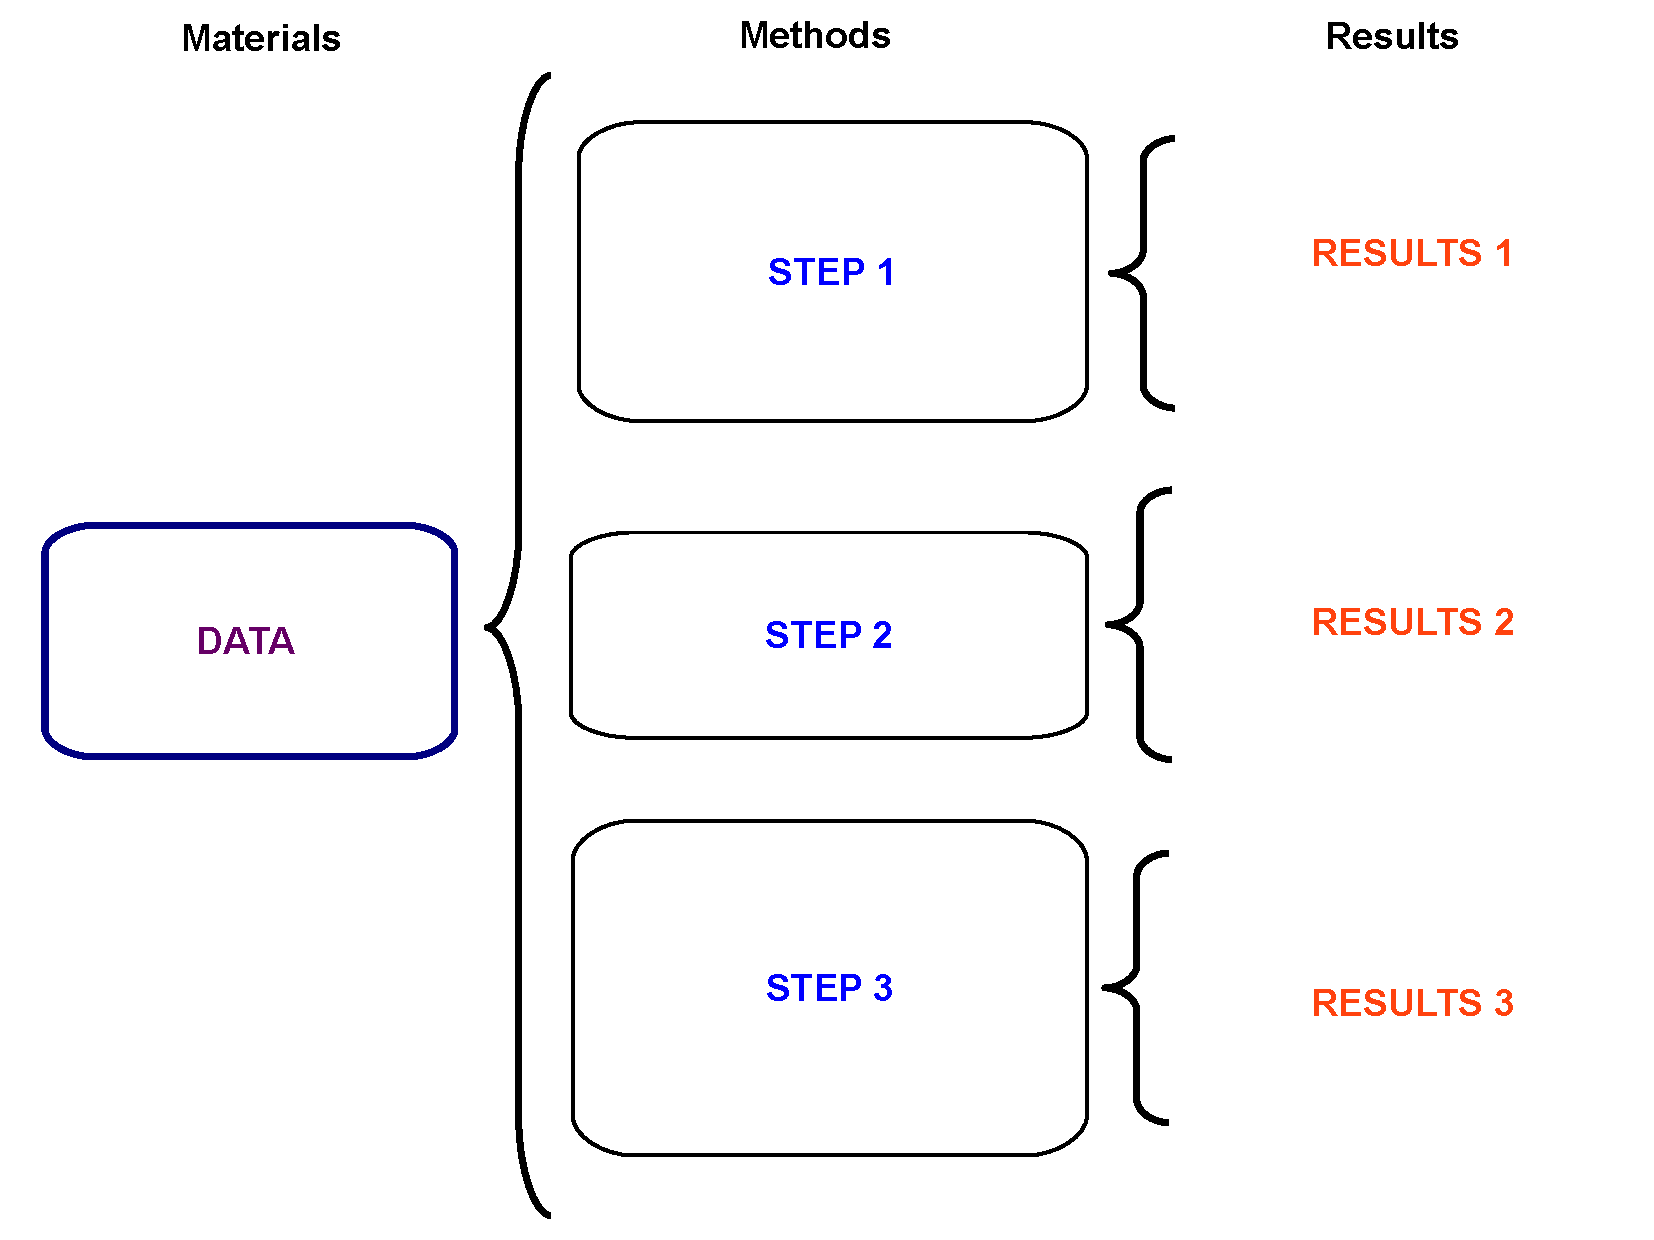
\includegraphics[width=0.9\columnwidth]{materials_and_methods/methods_diagram.pdf}
        \end{center}
    \caption[Flux diagram of general methodology]{
    \textit{\textbf{Flux diagram of general methodology} 
      }
    }
    \label{fig_methods_flux_diagram}    
\end{figure}


		% ***************************************
% ***************************************
\chapter{Results} \label{results}
% ***************************************
% ***************************************

The infinite monkey theorem states that a monkey hitting keys at random on a typewriter keyboard for an infinite amount of time will almost surely type a given text, such as the complete works of William Shakespeare.
\\
\\
In this context, \textit{almost surely} is a mathematical term with a precise meaning, and the \textit{monkey} is not an actual monkey, but a metaphor for an abstract device that produces an endless random sequence of letters and symbols. One of the earliest instances of the use of the \textit{monkey metaphor} is that of French mathematician Émile Borel in 1913 \cite{borel1913mecanique}, but the earliest instance may be even earlier. The relevance of the theorem is questionable—the probability of a universe full of monkeys typing a complete work such as Shakespeare's Hamlet is so tiny that the chance of it occurring during a period of time hundreds of thousands of orders of magnitude longer than the age of the universe is extremely low (but technically not zero).
\\
\\
Variants of the theorem include multiple and even infinitely many typists, and the target text varies between an entire library and a single sentence. The history of these statements can be traced back to Aristotle's On Generation and Corruption and Cicero's De natura deorum (On the Nature of the Gods), through Blaise Pascal and Jonathan Swift, and finally to modern statements with their iconic simians and typewriters. In the early 20th century, Émile Borel and Arthur Eddington used the theorem to illustrate the timescales implicit in the foundations of statistical mechanics \cite{wikiMonkeys}.

\newpage
Table \ref{table_monkeys_vs_bananas} shows the number of bananas eaten by each electronic monkey tested:

\begin{table}[h!]
    \begin{center}
        \begin{tabular}{|c|c|}
        \hline
        \textbf{Monkey}  &  \textbf{Bananas eaten} \\ \hline
        1   &   2  \\ \hline
        2   &   3  \\ \hline
        3   &   6  \\ \hline
        4   &   15  \\ \hline
        5   &   6  \\ \hline
        6   &   8  \\ \hline
        7   &   2  \\ \hline
        8   &   4  \\ \hline
        9   &   9  \\ \hline
        10  &   4  \\ \hline
        \end{tabular}
    \end{center}
  \caption{Monkeys vs bananas}
  \label{table_monkeys_vs_bananas}
\end{table}

Figure \ref{fig_monkeys_vs_bananas} shows the same as table \ref{table_monkeys_vs_bananas}:

% insert figure
\begin{figure}[h!]
        \begin{center}
        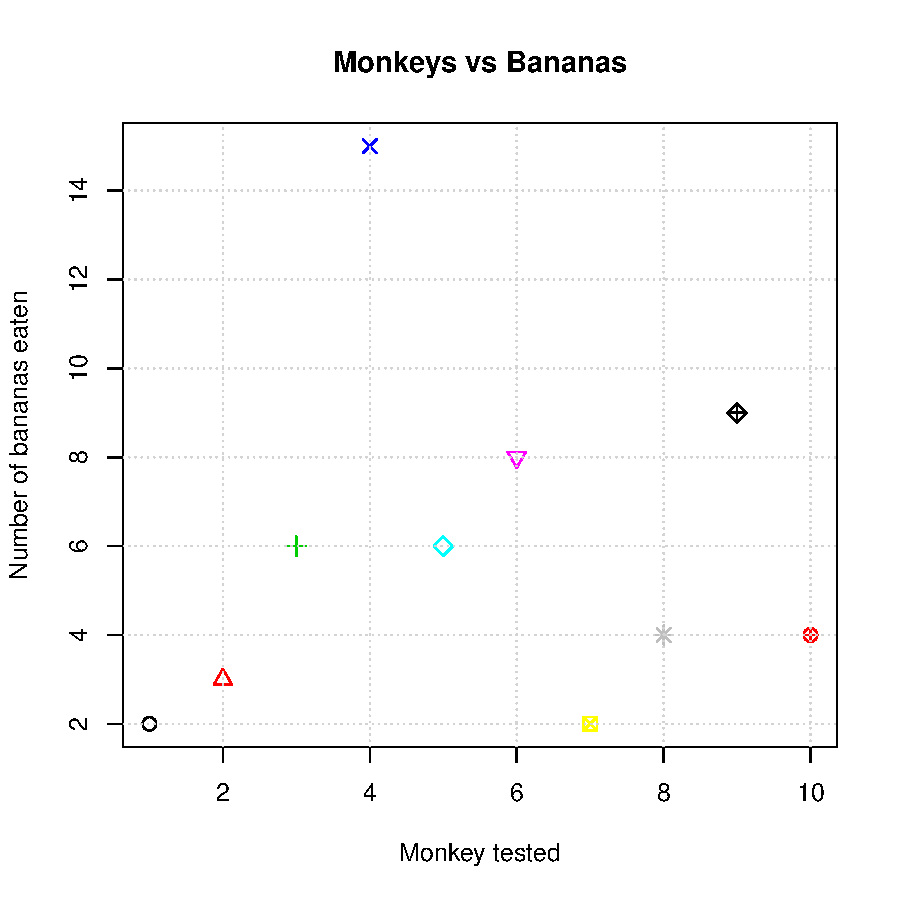
\includegraphics[width=0.7\columnwidth]{results/monkeys_vs_bananas.pdf}
        \end{center}
    \caption[Monkeys vs bananas eaten]{
    \textit{\textbf{Monkeys vs bananas eaten} 
      }
    }
    \label{fig_monkeys_vs_bananas}    
\end{figure}


		% ***************************************
% ***************************************
\chapter{Discussion} \label{discussion}
% ***************************************
% ***************************************

The infinite monkey theorem states that a monkey hitting keys at random on a typewriter keyboard for an infinite amount of time will almost surely type a given text, such as the complete works of William Shakespeare.
\\
\\
In this context, \textit{almost surely} is a mathematical term with a precise meaning, and the \textit{monkey} is not an actual monkey, but a metaphor for an abstract device that produces an endless random sequence of letters and symbols. One of the earliest instances of the use of the \textit{monkey metaphor} is that of French mathematician Émile Borel in 1913 \cite{borel1913mecanique}, but the earliest instance may be even earlier. The relevance of the theorem is questionable—the probability of a universe full of monkeys typing a complete work such as Shakespeare's Hamlet is so tiny that the chance of it occurring during a period of time hundreds of thousands of orders of magnitude longer than the age of the universe is extremely low (but technically not zero).
\\
\\
Variants of the theorem include multiple and even infinitely many typists, and the target text varies between an entire library and a single sentence. The history of these statements can be traced back to Aristotle's On Generation and Corruption and Cicero's De natura deorum (On the Nature of the Gods), through Blaise Pascal and Jonathan Swift, and finally to modern statements with their iconic simians and typewriters. In the early 20th century, Émile Borel and Arthur Eddington used the theorem to illustrate the timescales implicit in the foundations of statistical mechanics \cite{wikiMonkeys}.

 
		% ***************************************
% ***************************************
\chapter{Conclusions and future work} \label{conclusions}
% ***************************************
% ***************************************

In this chapter, the conclusions derived from the results 
(chapter \ref{results}) are shown in section \ref{section_conclusions}. 
Additionally, future work and suggestions to extend the current investigation are shown in 
section \ref{section_future_work}. 

% ***************************************
\section{Conclusions} \label{section_conclusions}
% ***************************************

Evolutionary algorithms are helpful to solve optimization problems. 
We conclude that the hypothesis proposed (see section \ref{hypothesis}) is true, our 
evidence is that we solved the infinite monkey problem. 
\\
\\
As a final comment, we expect that experimental and computational 
advances will lead to better modeling and understanding of typing monkeys. 

% ***************************************
\section{Future work} \label{section_future_work}
% ***************************************

There are some research questions arising from this work which should be addressed.

\begin{itemize}
	\item \textbf{Get real monkeys:} In order 
	to test experimentally our hypothesis, real monkeys are needed.
	\item \textbf{Pursue a scientific publication}.
\end{itemize}



	%%%%%%%%%%%%%%%%%%%%%%%%%%%%%%%%%%%%%%%%%%%%%%%%%%%%%%%%%%%%%%%%%%%%%%%%%%%%%%%%
	% Load bibliography style :
	% ieeetr is IEEE format
		\bibliographystyle{ieeetr}
	% Load bibliography file :
		\bibliography{bibliography/references}
	%%%%%%%%%%%%%%%%%%%%%%%%%%%%%%%%%%%%%%%%%%%%%%%%%%%%%%%%%%%%%%%%%%%%%%%%%%%%%%%%
	% add vita
		% ***************************************
% ***************************************
\chapter*{Vita} \label{Vita}
% ***************************************
% ***************************************

\addcontentsline{toc}{chapter}{Vita}

%%%%%%%%%%%%%
\begin{center}
\end{center}
%%%%%%%%%%%%%

\authorName\ is a fictional character and  
protagonist of the comic science fiction series The Hitchhikers
 Guide to the Galaxy by Douglas Adams. 
Sadly, he was not accepted in the graduate programs in Information Technologies  
on January 2013 at Instituto Tecnológico y de Estudios Superiores de 
Monterrey, Monterrey Campus.

%%%%%%%%%%%%%
\begin{center}
\end{center}
%%%%%%%%%%%%%

\begin{center}
	{@}\thesisYear\ by \authorName \\
	All rights reserved
\end{center}

\null
\vfill

% insert footnote with package details
\begin{center}
	\packageDetails
\end{center}

\begin{center}
    \textbf{\thesisDate} 
\end{center}



	%%%%%%%%%%%%%%%%%%%%%%%%%%%%%%%%%%%%%%%%%%%%%%%%%%%%%%%%%%%%%%%%%%%%%%%%%%%%%%%%
\end{document}


